\section{Odds Ratio}
In lecture 9, we assume the rows of contingency table are two independent binomial distributions, and we would like to check whether the two distribution have the same probability parameter.

In this lecture, we would like to exam the dependency. For conditional design, we check the dependency between the two binomial distribution for each row. For the unconditional design, we check the dependency among the four cells in the table.One common used measure for association/dependency is the sample odds ratio.

\subsection{Odds}
For a probability of success $\pi_1$, the odds of success are defined to be $\pi_1 / (1 - \pi_1)$. For instance, if $\pi_1 = 0.75$, the odds of success equal 3.

The odds are non-negative, with value greater than 1 when a success is more likely than a failure.
\begin{itemize}
	\item When odd = $3$, a success is 3 times as likely as a failure. We expect to observe 3 successes for every 1 failure.
	\item When odd = $1/3$, a failure is 3 times as likely as a success. We expect to observe 1 success for every 3 failure.
\end{itemize}

\subsection{Odds Ratio}
Suppose
\begin{itemize}
	\item Random variable $U$ has probability of success $\pi_1$.
	\item Random variable $V$ has probability of success $\pi_2$.
\end{itemize}
\begin{definition}[Odds Ratio]
	Odds ratio is the ratio of two odds
	\[\theta = \frac{\frac{\pi_1}{1 - \pi_1}}{\frac{\pi_2}{1 - \pi_2}} \ge 0\]
\end{definition}

If $\pi_1 = \pi_2$, then $\theta = 1$. The independence of $U$ and $V$ $\iff$ $\theta = 1$.

\subsection{Conditional Design}
Suppose the treatment group subjects iid Bernoulli($\pi_1$), $i = 1, \cdots, n_1$, and the control group subjects iid Bernoulli($\pi_2$), $j = 1, \cdots, n_2$.
\begin{figure}[H]
	\centering
	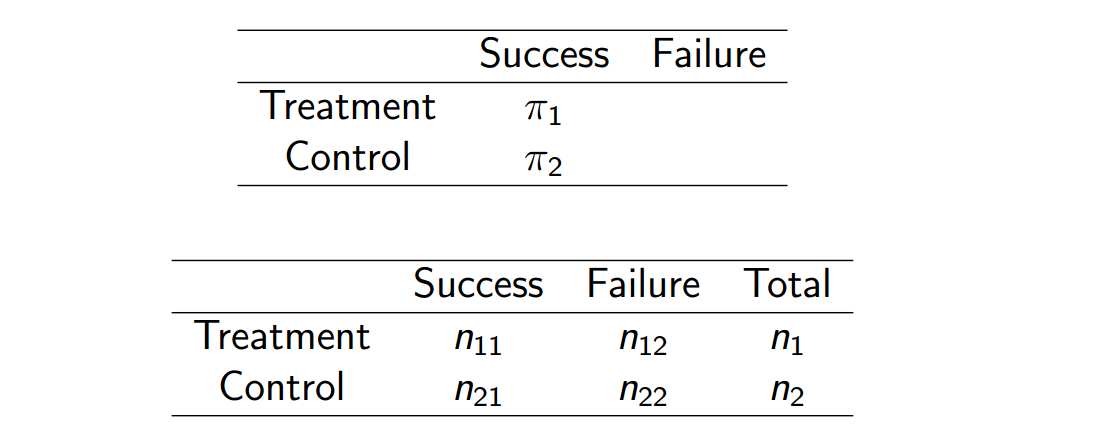
\includegraphics[width=0.7\linewidth]{fig/screenshot001}
	\caption{Conditional Contingency Table}
	\label{fig:screenshot001}
\end{figure}

The sample odd ratio is 
\[\hat{\theta} = \frac{\frac{\pi_1}{1 - \pi_1}}{\frac{\pi_2}{1 - \pi_2}} = \frac{\frac{n_{11}}{n_{12}}}{\frac{n_{21}}{n_{22}}} = \frac{n_{11}n_{22}}{n_{12}n_{21}}\]

\subsection{Unconditional Design}
Let $\pi_{ij}$ denote the true unknown joint probability of falling into the $ij$-th cell, $i=1,2$, $j=1,2$. The contingency table is as follows.

\begin{figure}[H]
	\centering
	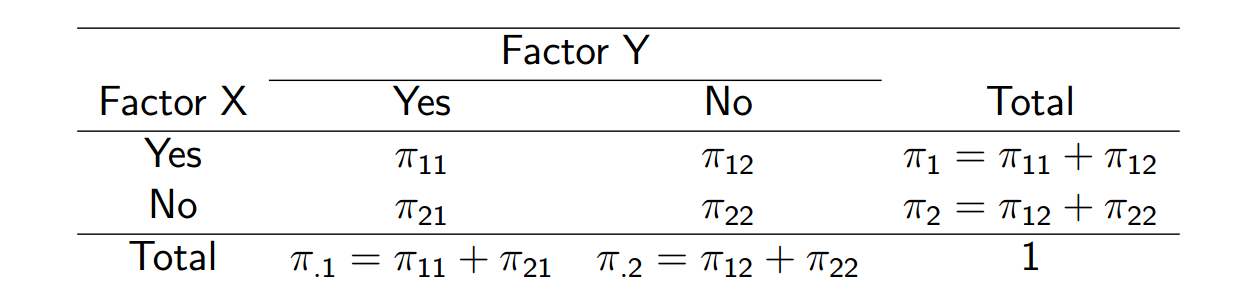
\includegraphics[width=0.7\linewidth]{fig/screenshot002}
	\caption{Unconditional Contingency Table}
	\label{fig:screenshot002}
\end{figure}

In the table, 
\begin{itemize}
	\item $\pi_{11} = \P(X = 1 \text{ and } Y = 1)$
	\item $\pi_{12} = \P(X = 1 \text{ and } Y = 1)$
	\item $\pi_{21} = \P(X = 0 \text{ and } Y = 1)$
	\item $\pi_{22} = \P(X = 0 \text{ and } Y = 0)$
\end{itemize}

The odd $\theta_1$ in the first row is 
\[\theta_1 = \frac{\P(Y = 1 | X = 1)}{P(Y = 0 | X = 1)} = \frac{\frac{\P(Y = 1, X = 1)}{\P(X = 1)}}{\frac{\P(Y = 0, X = 1)}{\P(X = 1)}} = \frac{\frac{\pi_{11}}{\pi_{11} + \pi_{12}}}{\frac{\pi_{12}}{\pi_{11} + \pi_{12}}} = \frac{\pi_{11}}{\pi_{12}}\]

The odd $\theta_2$ in the second row is 
\[\theta_2 = \frac{\P(Y = 1 | X = 0)}{P(Y = 0 | X = 0)} = \frac{\frac{\P(Y = 1, X = 0)}{\P(X = 0)}}{\frac{\P(Y = 0, X = 0)}{\P(X = 0)}} = \frac{\frac{\pi_{21}}{\pi_{21} + \pi_{22}}}{\frac{\pi_{22}}{\pi_{21} + \pi_{22}}} = \frac{\pi_{21}}{\pi_{22}}\]

Therefore, the population odd ratio is
\[\theta = \frac{\theta_1}{\theta_2} = \frac{\frac{\pi_{11}}{\pi_{12}}}{\frac{\pi_{21}}{\pi_{22}}} = \frac{\pi_{11}\pi_{22}}{\pi_{21}\pi_{22}}\]
Hence, the sample odd ratio is
\[\hat{\theta} = \frac{n_{11}n_{22}}{n_{21}n_{22}}\]

One may notice that the sample odd ratios are the same in two different studies.